\section{Specifying Parity Games}
\label{sec:specs}

\pgsolver expects the parity game it should solve or display to be given in its own
specification language. There, a parity game consists of an optional \emph{header line} and
a list of \emph{node specifications}. The header line tells \pgsolver the highest
occurring identifier in the game helping to speed up the parsing process. Each
node specification contains an identifier of a node (a natural number), its priority, the
player who owns the node, the list of its successors and, optionally, a symbolic
name of the node. The format can easily be described in EBNF. 
\begin{align*}
\nonterminal{parity\_game} \enspace &::= \enspace [\terminal{parity} \enspace \nonterminal{identifier} \enspace \terminal{;}] \enspace \nonterminal{node\_spec}^+ \\[2mm]
\nonterminal{node\_spec} \enspace &::= \enspace \nonterminal{identifier} \enspace
  \nonterminal{priority} \enspace \nonterminal{owner} \enspace \nonterminal{successors}
  \enspace [\nonterminal{name}] \enspace \terminal{;} \\[2mm]
\nonterminal{identifier} \enspace &::= \enspace \Nat \\[2mm]
\nonterminal{priority} \enspace &::= \enspace \Nat \\[2mm]
\nonterminal{owner} \enspace &::= \enspace \terminal{0} \mid \terminal{1} \\[2mm]
\nonterminal{successors} \enspace &::= \enspace \nonterminal{identifier}\enspace
  (\terminal{,}\enspace \nonterminal{identifier})^* \\[2mm]
\nonterminal{name} \enspace &::= \enspace \texttt{"}\enspace
  (\mbox{ any ASCII string not containing `{\texttt{"}}'}) \enspace \texttt{"}
\end{align*}
There must be whitespace characters between the following pairs of tokens:
\nonterminal{identifier} and \nonterminal{priority}, \nonterminal{priority} and \nonterminal{owner},
\nonterminal{owner} and \nonterminal{identifier}.

The \textit{identifier} -- in effect a natural number -- that is given at the beginning of
the specification after the keyword \texttt{parity} allows more efficient parsing. It should be the
maximal identifier of a node in the game. If it is smaller, parsing will fail. If it is bigger
then parsing will be successful and solving should be possible as well, but internally the game
will be blown up with undefined nodes. For large games we recommend adding the 
\texttt{parity}\ \nonterminal{identifier} at the beginning. Note that currently, the old format
without the size specification is still supported but may be dropped in a future version of
\pgsolver.

In order to give a precise semantics to this syntax we introduce the following notation. Let
$G = (V,V_0,V_1,E,\Omega)$ be a parity game with $V \subseteq \Nat$, and
$\alpha := (v,p,i,s) \in \Nat \times \Nat \times \{0,1\} \times \Nat^+$. Then $G + \alpha$
is defined as the parity game $(V',V'_0,V'_1,E',\Omega')$ where
\begin{align*}
V' \enspace &:= \enspace V \cup \{v\} \\
V'_0 \enspace &:= \enspace V_0 \cup \begin{cases} \{v\} &, \mbox{ if } i=0 \\
     \emptyset &, \mbox{otherwise} \end{cases} \\
V'_1 \enspace &:= \enspace V_1 \cup \begin{cases} \{v\} &, \mbox{ if } i=1 \\
     \emptyset &, \mbox{otherwise} \end{cases} \\
E' \enspace &:= \enspace (E \cap (V \setminus \{v\})^2) \cup \{ (v,w) \mid s = \ldots,w,\ldots \} \\
\Omega'(w) \enspace &:= \enspace \begin{cases} p &, \mbox{ if } w=v \\
     \Omega(w) &, \mbox{otherwise} \end{cases}
\end{align*}
Now let $G_0 := (\emptyset,\emptyset,\emptyset,\emptyset,\bot)$ with $\bot$ being the empty
function. Then we can recursively define the semantics of a parity game specification as follows.
Let $\epsilon$ denote the empty list of node specifications.
\begin{align*}
\sem{\epsilon} \enspace &:= \enspace G_0 \\
\sem{l\, (\mathtt{v\, p\, i\, s\, n;})} \enspace &:= \enspace \sem{l} + (v,p,i,s) \\
\sem{l\, (\mathtt{v\, p\, i\, s;})} \enspace &:= \enspace \sem{l} + (v,p,i,s) \\
\end{align*}
Note that the EBNF definition of the syntax does not ensure well-formedness of a parity game.
For instance, one can list identifiers in the successors list of a node that do not have node
specifications for themselves. \pgsolver assumes the input games to be well-formed in that sense.
Otherwise it will terminate with an error message.

\begin{figure}[t]
\begin{center}
\scalebox{0.6}{%\includegraphics{graphics/examplegame.ps}}
\begin{tikzpicture}[very thick,-triangle 45,start chain=circled placed {at=(\tikzchaincount*72:6)}]

  \tikzstyle{boxnode}=[draw=black,shape=rectangle,inner sep=10pt]
  \tikzstyle{diamnode}=[draw=black,very thin,shape=diamond]

  \node[on chain,diamnode] (australia)  {Australia: 6};
  \node[on chain,diamnode] (asia)       {Asia: 7};
  \node[on chain,boxnode]  (africa)     {Africa: 6};
  \node[on chain,boxnode]  (antarctica) {Antarctica: 5};
  \node[on chain,boxnode]  (america)    {America: 8};

  \path (america)    edge                (australia)
                     edge [bend left=5]  (asia)
                     edge                (antarctica)
        (australia)  edge [bend left=10] (asia)
                     edge                (antarctica)
        (antarctica) edge [bend left=10] (africa)
        (africa)     edge [bend left=10] (antarctica)
                     edge [bend left=10] (asia)
        (asia)       edge [bend left=10] (australia)
                     edge [bend left=5]  (america)
                     edge [bend left=10] (africa)
                     edge                (antarctica);
\end{tikzpicture}}
\end{center}

\caption{An example of a parity game.}
\label{fig:examplegame}
\end{figure}

\begin{example}
\label{ex:examplegame}
The parity game depicted in Fig.~\ref{fig:examplegame} can, for example, be specified as follows.
\begin{verbatim}
     parity 4;
     0 6 1 4,2 "Africa";
     4 5 1 0 "Antarctica";
     1 8 1 2,4,3 "America";
     3 6 0 4,2 "Australia";
     2 7 0 3,1,0,4 "Asia";
\end{verbatim}
Nodes belonging to player $0$ are shown in diamond shape, the others in box shape. The label in each
node is composed of the node's name and its priority. Note that symbolic names are optional.
\end{example}

Currently, parity games are stored as arrays of node specifications. The index in that array at which
a node is stored, equals its identifier. This has two important and noteworthy consequences.
\begin{itemize}
\item As noted above, using identifiers multiply leads to overriding of nodes. If the parity game
      contains more than one node specification with the same identifier then the \emph{last} node
      specification determines the properties of the node with that index.
\item The size of the array that is allocated to store a parity game is always $n+1$ where $n$ is
      the maximal identifier occurring in the game's specification. To avoid unnecessary waste of
      space you should ensure that the nodes' identifiers in a parity game occupy a closed interval
      of the natural numbers of the form $\{0,1,2,\ldots,n\}$.
\end{itemize}



%%% Local Variables:
%%% mode: latex
%%% TeX-master: "main"
%%% End:
